\documentclass[a4paper]{article}
\usepackage[slovene]{babel}
\usepackage[T1]{fontenc}
\usepackage[utf8]{inputenc}
\usepackage{lmodern}
\usepackage{amsfonts}
\usepackage{amsmath}
\usepackage{makeidx}
\usepackage{graphicx}
\graphicspath{ {./images/} }



\title{Finančni praktikum \\\vspace{2cm} {\huge $k$-total rainbow domination numer vs. domination number}\vspace{2cm}}
\author{Tim Resnik \\[1.5mm] Lana Herman \\[1.5mm]\vspace{6cm}
Univerza v Ljubljani \\[1.5mm]
Fakulteta za matematiko in fiziko \vspace{2cm}}
\date{November, 2019}

\begin{document}

\begin{titlepage}
\clearpage \maketitle
\thispagestyle{empty}
\end{titlepage}

\section{Problem naloge}

V projektni nalogi se bova ukvarjala z domeno, ki se ukvarja s povezavo med "k-rainbow total domination number" (označimo z $\gamma_{krt}(G)$)  in "domination number" (označimo z $\gamma(G)$). Definiciji za $\gamma_{krt}(G)$ in $\gamma(G)$ sta v razdelku \textbf{Razlaga pojmov}.\\
Domneva pravi, da za graf G in $k \geq 4$ \text{obstaja tesna povezava} $\gamma_{krt}(G) \geq 2\gamma(G)$. Cilj najine projetkne naloge je najti tak graf, za katerega ta neenkost ne drži. To sva na majhnih grafih preverila na konkretnih primerih, kjer sva število vozlišč in število $k$ vnesla ročno. Za večje grafe sva uporabila metodo \textit{Simulated Annealing}.\\
Poiskala sva tudi primere, za katere velja enakost $\gamma_{krt}(G) = 2\gamma(G)$.

\section{Razlaga pojmov}

Graf $G$ ima množico vozlišč $V(G)$ in množico povezav $E(G)$. Za množico $N_G(v)$ velja, da vsebuje vsa sosednja vozlišča $v$, v grafu G. Za grafa G in H, je kartezični produkt $G \square H$ graf z množico vozlišč $V(G) \times V(H)$.\\
\textit{Dominirana množica} grafa $G$ je $D \subseteq V(G)$, taka da za vsako vozlišče $v \in V(G)$ in $v \notin D$ velja, da je sosed nekemu vozlišču iz $D$. \textit{Dominirano število}, $\gamma(G)$, je velikost najmanjše dominirane množice. Če za $\forall v \in V(G)$ velja, da je sosed vozlišču iz $D$, za $D$ rečemo, da je \textit{totalno dominirana množica} grafa $G$. \textit{Totalno dominirano število}, $\gamma_{t}(G)$, je velikost najmanjše totalno dominirane množice.\\
Za pozitivno celo število $k$, je \textit{"k-rainbow domination function"} ($k$RDF) grafa $G$ funkcija $f$, ki slika iz $V(G)$ v množico $\{1, \cdots, k\}$. Zanjo velja, da za katerikoli $v \in V(G)$ in $f(v) = \emptyset$ velja $\cup_{u \in N_G(v)} f(u) = [k]$. Definiramo $\|f\| = \sum_{v \in V(G)}|f(v)|$. $\|f\|$ rečemo \textit{teža} $f$-a. \textit{"k-rainbow domination number"}, $\gamma_{kr}(G)$, grafa $G$ je minimalna vrednost $\|f\|$ za vse "k-rainbow domination functions". Po definiciji vemo, da za vse $k \geq 1$ velja $$\gamma_{kr}(G) = \gamma(G \square K_k).$$
Graf $K_k$ predstavlja polni graf na $k$ vozliščih. Nazadnje definirajmo še \textit{"k-rainbow total domination function"} ($k$RTDF), katera se od "k-rainbow domination function" razlikuje v dodatnem pogoju, ki zagotavlja, da če za $\forall v \in V(G)$ velja $f(v) = \{i\}$, potem obstaja tak $u \in N_G(v)$, da je $i \in f(u)$. \textit{"k-rainbow total domination number"}, $\gamma_{krt}(G)$, grafa $G$ je minimalna vrednost $\|f\|$ za vse "k-rainbow total domination functions". Tudi tu za vse $k \geq 1$ velja $$\gamma_{krt}(G) = \gamma_t(G \square K_k).$$
\pagebreak

\section{Reševanje problema}

\subsection{Majhni grafi}

\begin{figure}[h]
    \centering
    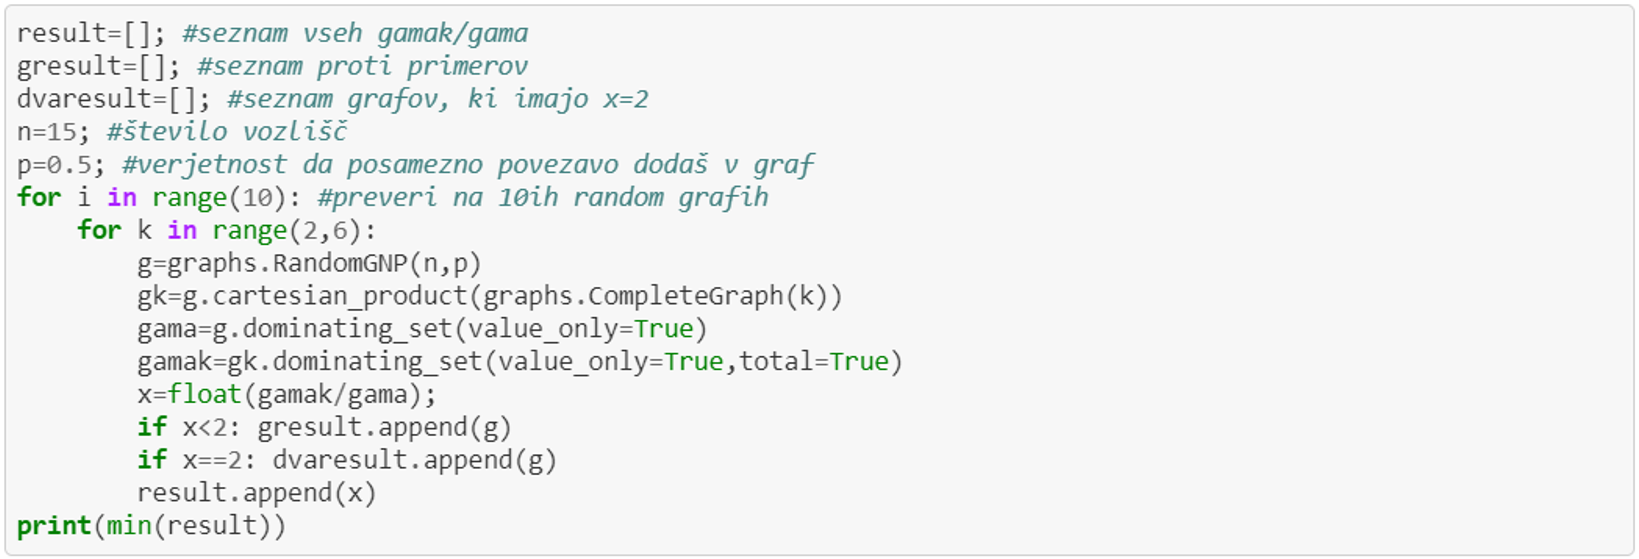
\includegraphics[width=13cm, height=5cm]{Slika1}
    \label{fig:mesh1}
\end{figure}

\begin{figure}[h]
    \centering
    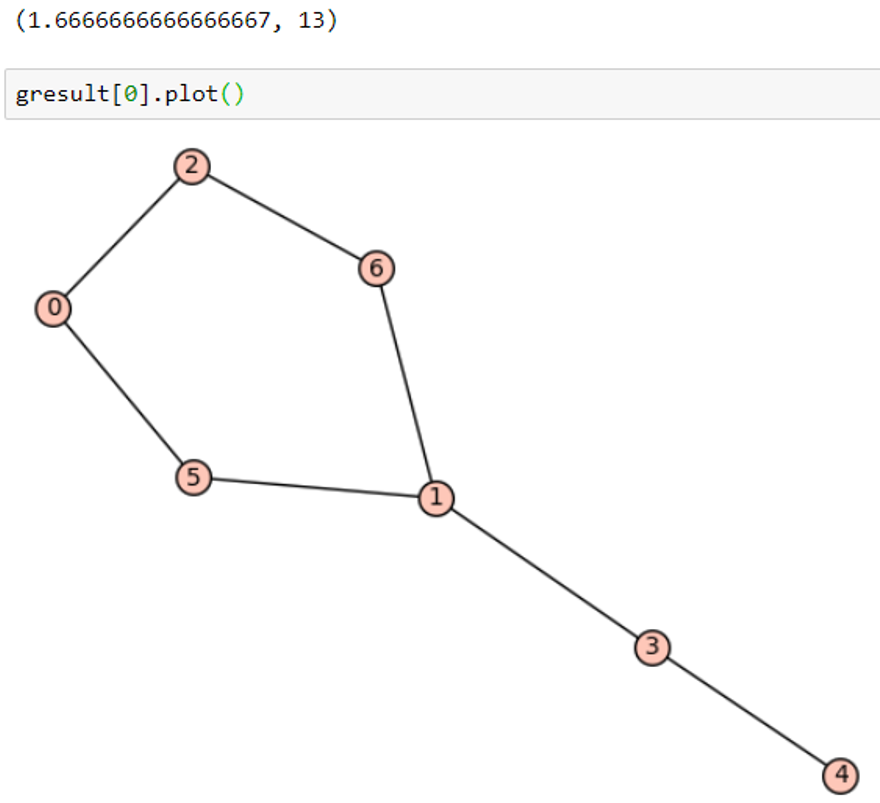
\includegraphics[width=12cm, height=13cm]{Slika2}
    \label{fig:mesh1}
\end{figure}

\begin{figure}[h]
    \centering
    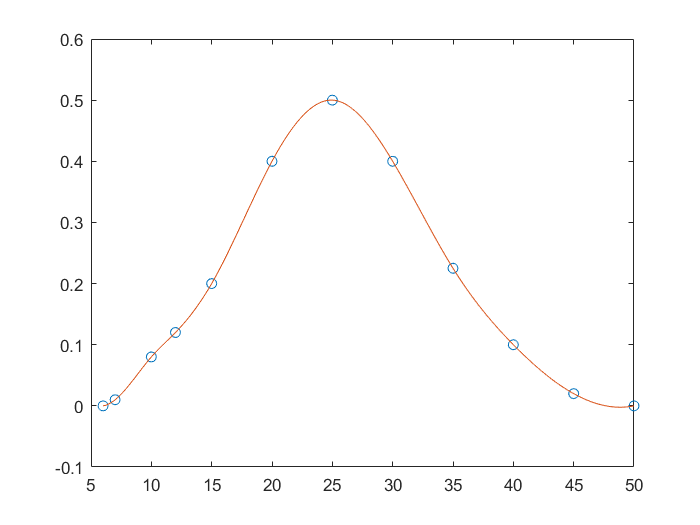
\includegraphics[width=12cm, height=15cm]{Slika3}
    \label{fig:mesh1}
\end{figure}


\end{document}